\subsection{Análisis de datos}
Relacionado al análisis exploratorio de datos, la Tabla \ref{tab:describe} muestra las métricas de estadistica descriptiva básica, donde podemos observar que a pesar de existir mínimos y máximos demasiado alejados entre sí, se puede asumir en primer lugar que el precio a lo largo de todo el tiempo ha presentado ligeras variaciones, teniendo una desviación estándar de $0.1037$ para la lactosa y $0.1325$ para el suero.

\begin{table}[htbp]
\centering
\caption{Estadistica descriptiva del precio de los productos.}
\begin{tabular}{lllll}
\hline
\multirow{2}{*}{Producto} & \multicolumn{4}{c}{Precio}          \\ \cline{2-5} 
                          & Promedio & Std    & Minimo & Máximo \\ \hline
Lactosa                   & 0.3873   & 0.1037 & 0.1925 & 0.6350 \\
Suero                     & 0.4404   & 0.1325 & 0.2350 & 0.8050 \\ \hline
\end{tabular}
\label{tab:describe}
\end{table}

Por otro lado, la Figura \ref{fig:distribuciones} muestra un análisis de distribución del precio en cada uno de los años analizados. Este análisis contradice la información del análisis estadístico básico, ya que muestra que en cada uno de los años sí se han presentando grande variaciones de precio, ya que los valores promedio de cada producto no están cerca de sí en cada uno de los años.

De igual forma se realizó un análisis de la variación de los precios de los productos por trimestre, se realizó por trimestre debido a que es un periodo muy común a analizar en diversas empresas. Este análisis se puede observar en la Figura \ref{fig:trimestres}, donde se refuerza el resultado del análisis de distribución por año, ya que se observa que trimestre a trimestre el precio ha mostrado variaciones muy grande, sin mostrar un valor constante entre todos ellos.

\begin{figure}[htbp]
\centering
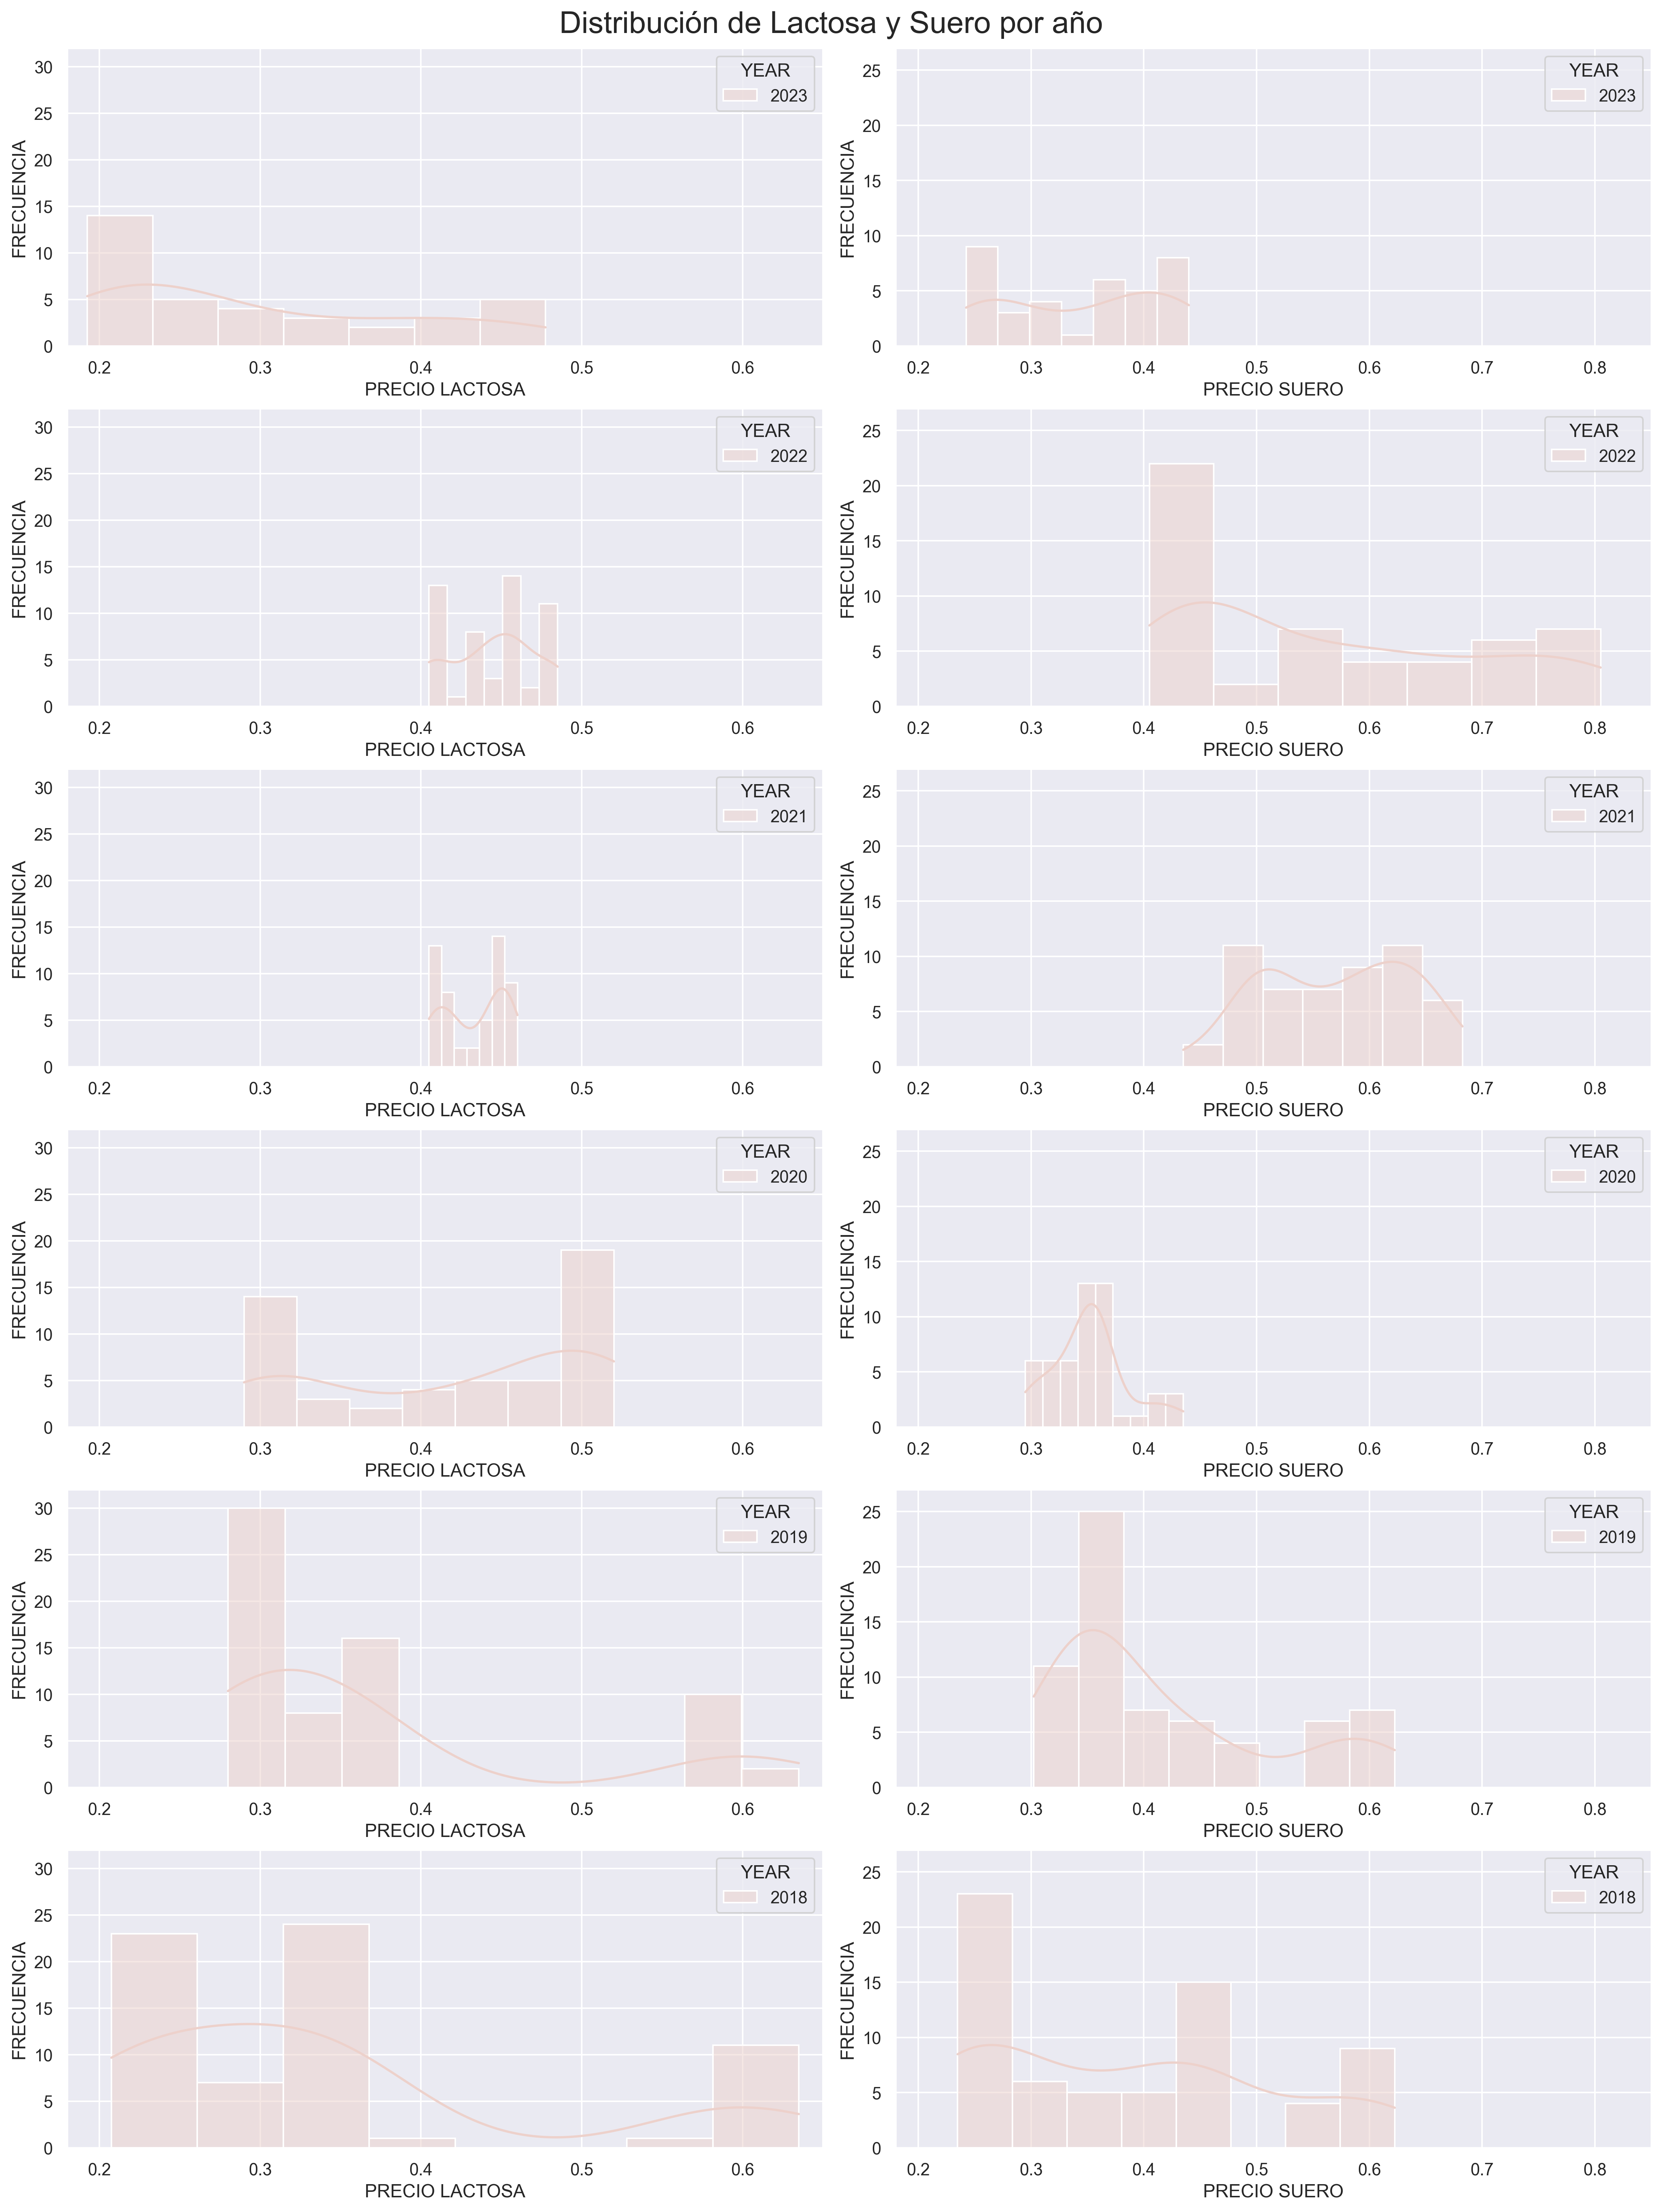
\includegraphics[width=0.8\textwidth]{distribuciones_precio}
\caption{Distribución de los precios de lactosa y suero en cada uno de los años analizados.}
\label{fig:distribuciones}
\end{figure}

\begin{figure}[htbp]
\centering
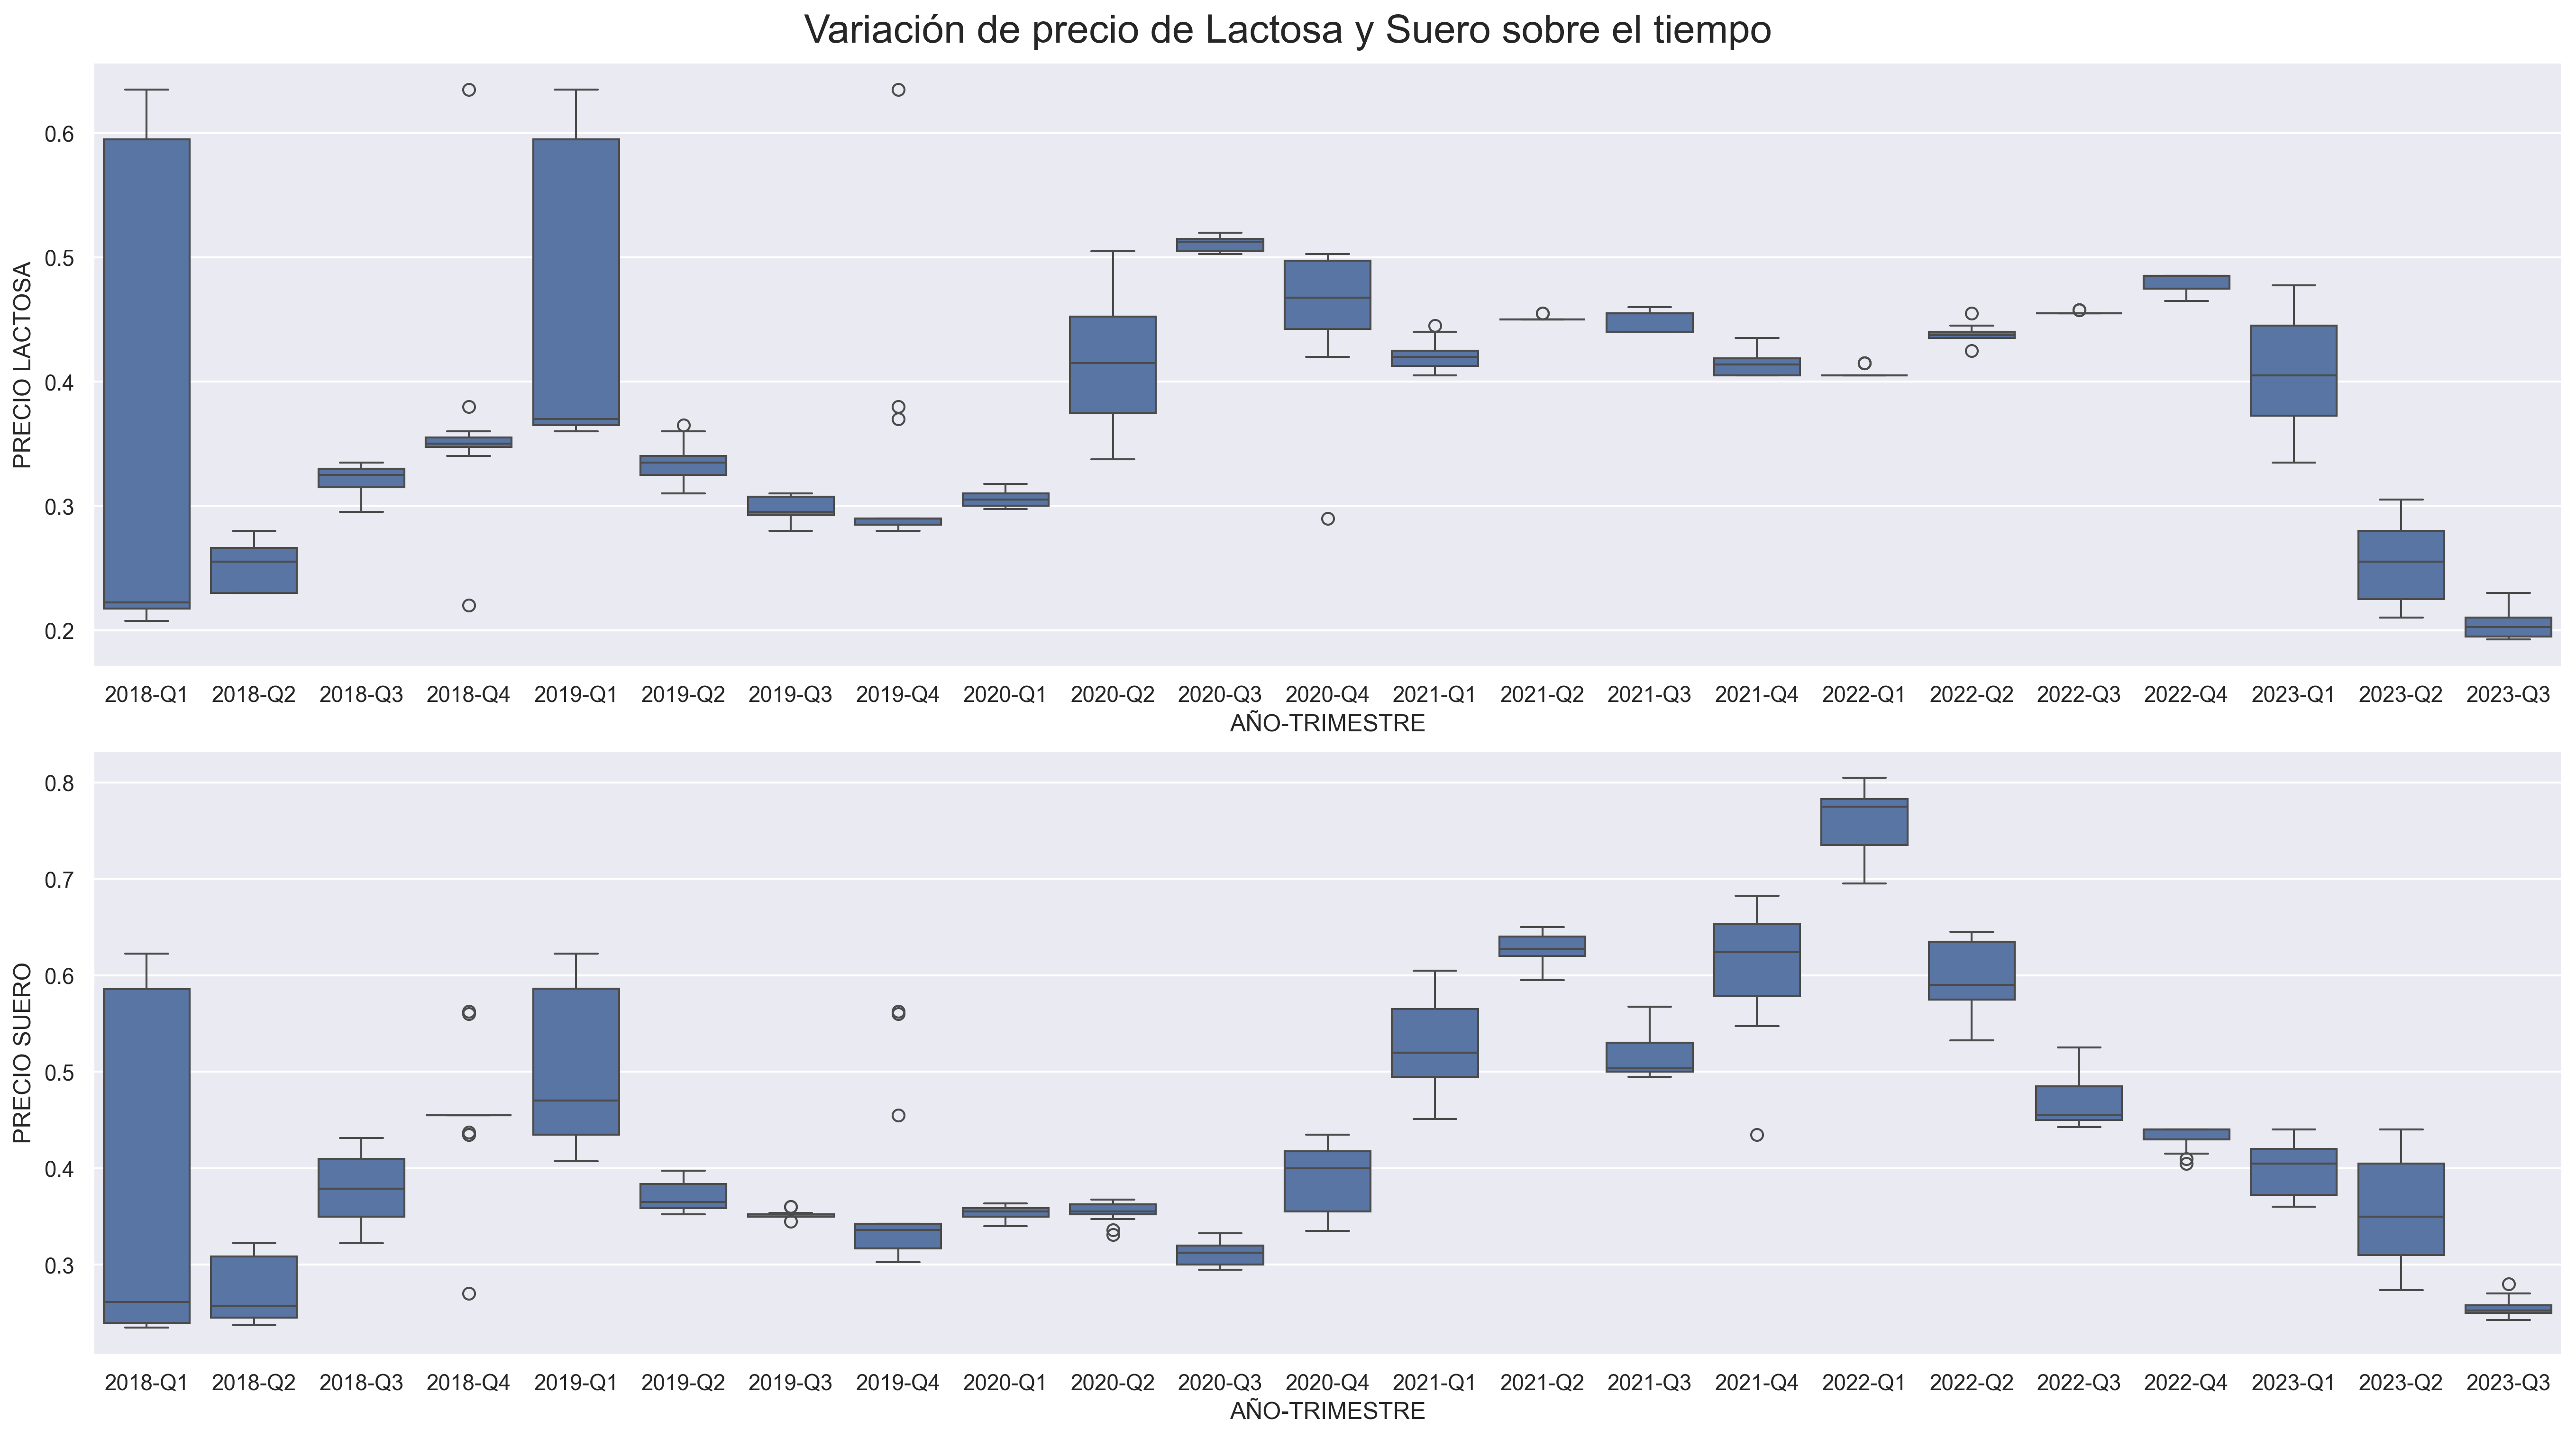
\includegraphics[width=\textwidth]{precio_tiempo}
\caption{Variación del precio de lactosa y suero en cada trimestre de los años analizados.}
\label{fig:trimestres}
\end{figure}


\FloatBarrier
\subsection{Funciones de aptitud}
Relacionado a la función de demanda de lactosa y suero, las Figuras \ref{fig:D_lactosa} y \ref{fig:D_suero} muestran el resultado de ajustar la ecuación lineal con los datos sintéticos de demanda/inventario.

\begin{figure}[htbp]
\centering
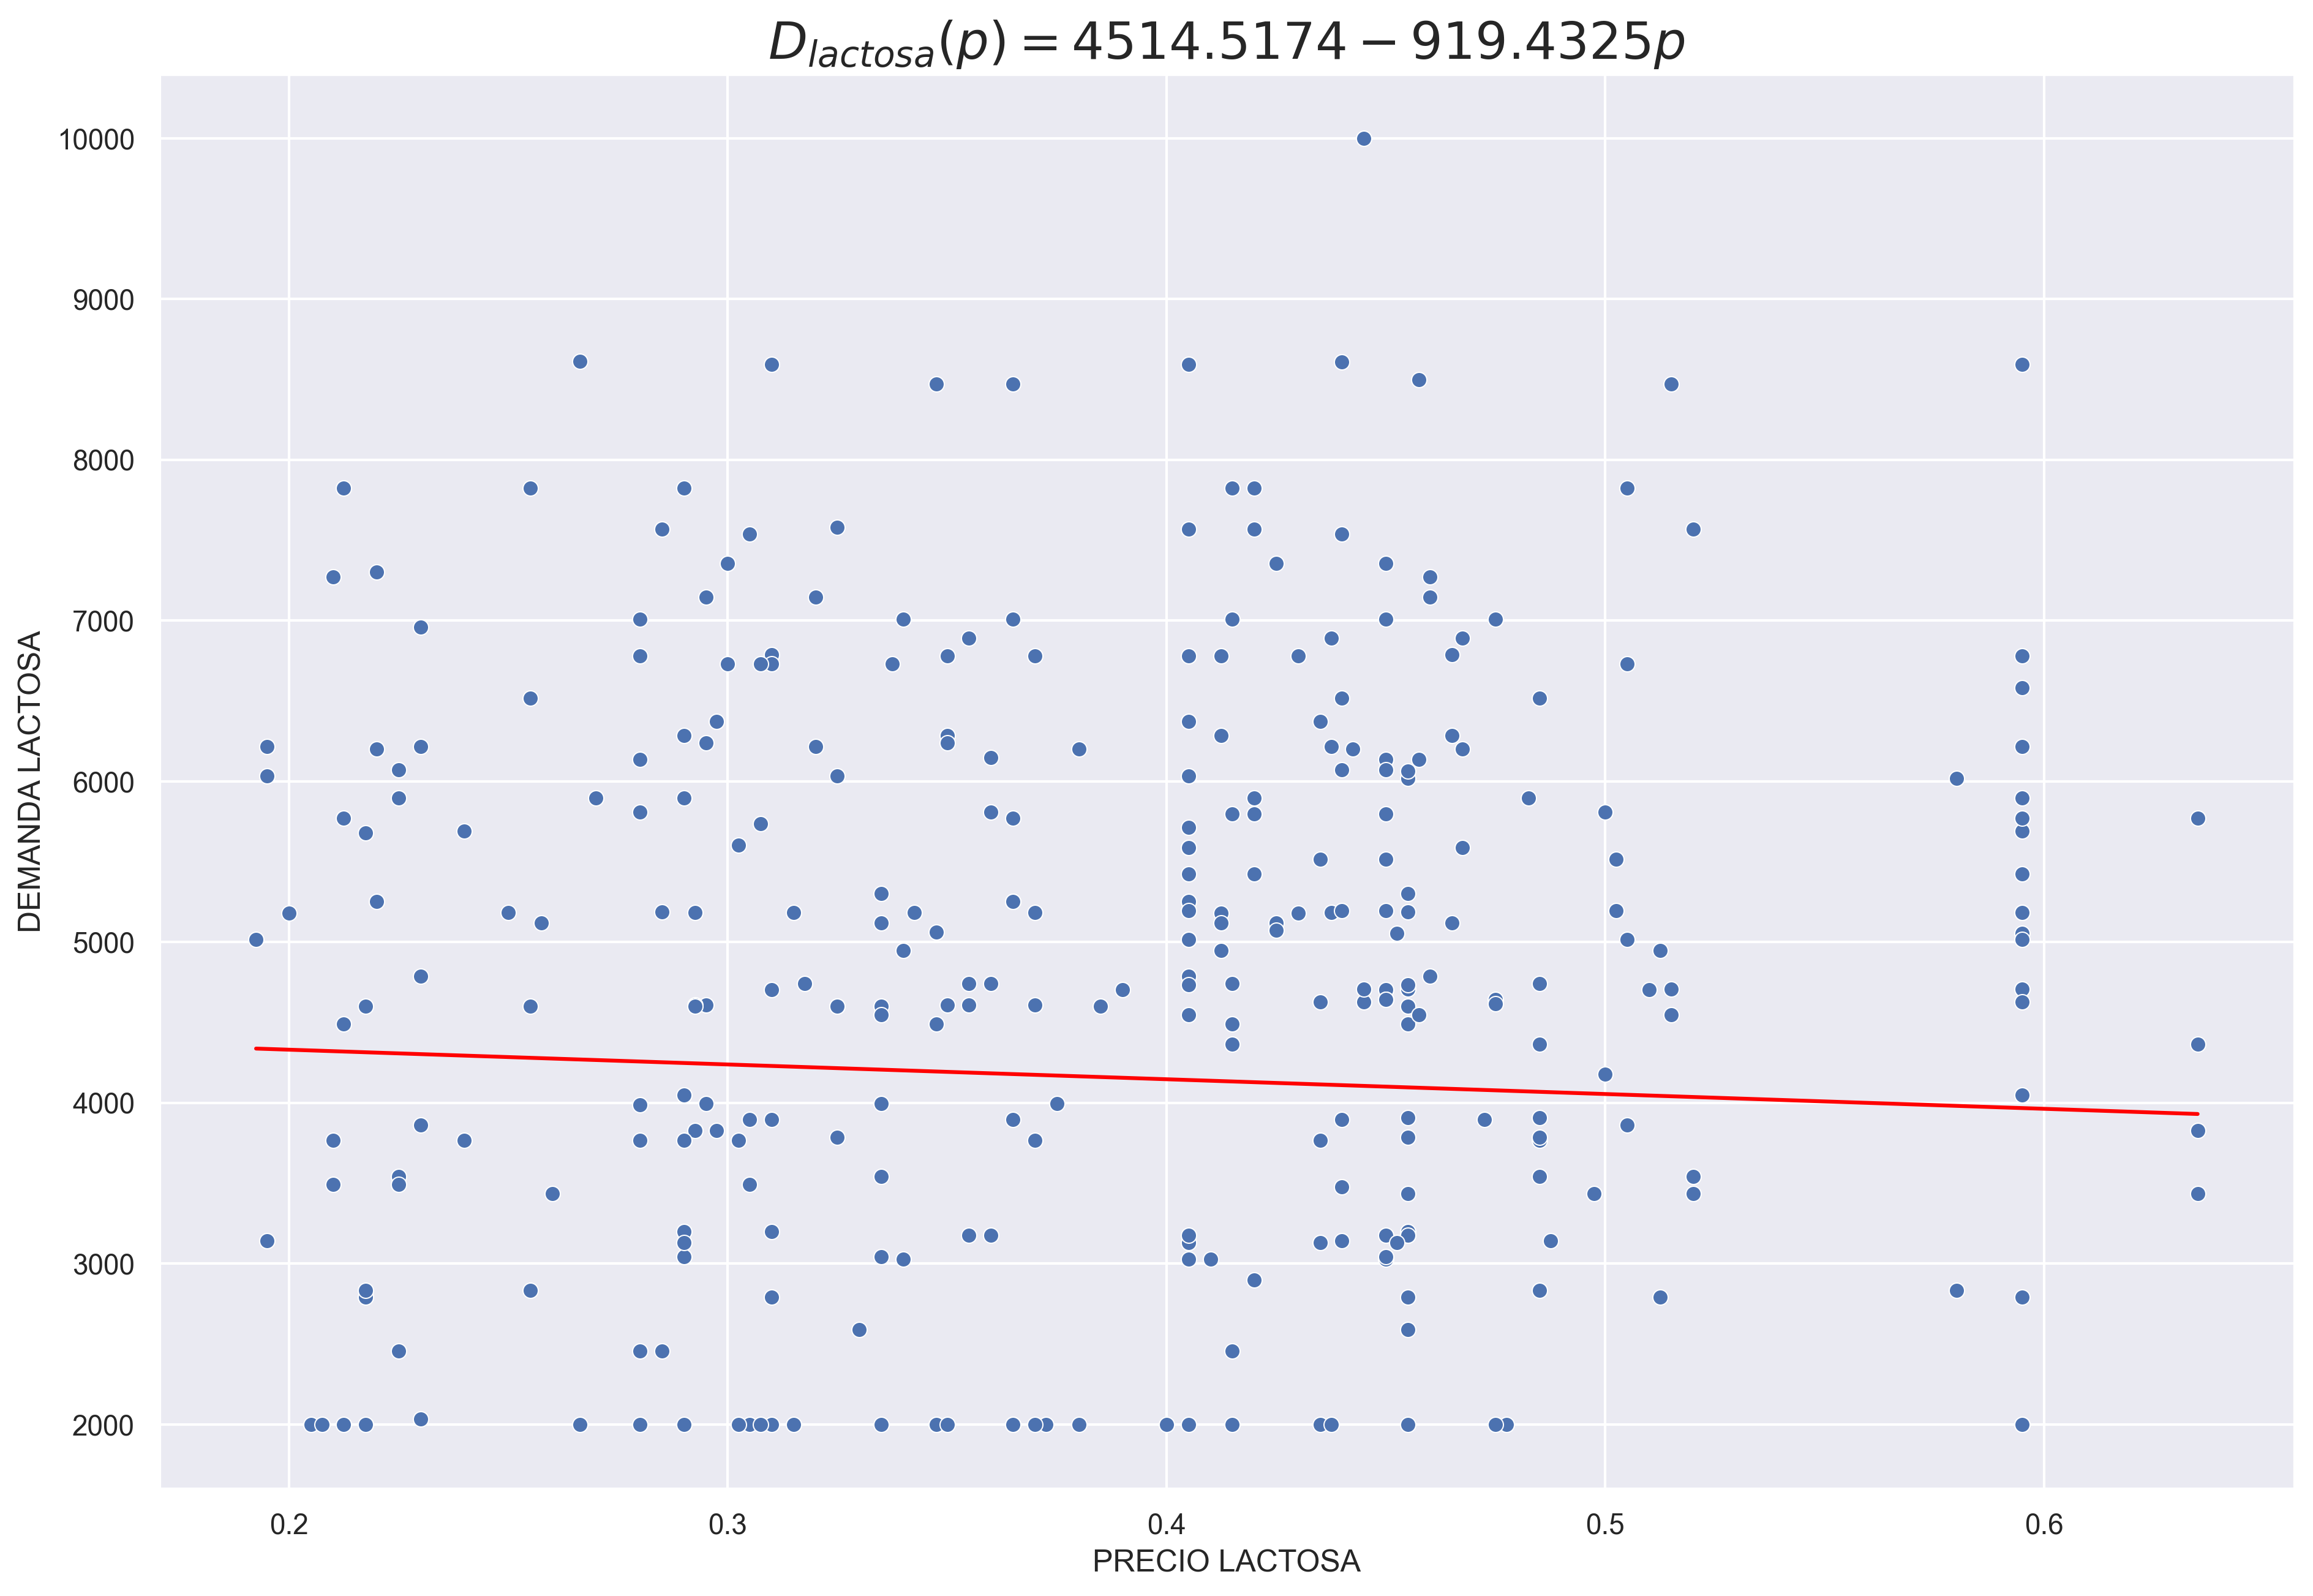
\includegraphics[width=0.7\textwidth]{demanda_lactosa}
\caption{Ecuación lineal ajustada a los datos sintéticos de demanda de lactosa.}
\label{fig:D_lactosa}
\end{figure}

\begin{figure}[htbp]
\centering
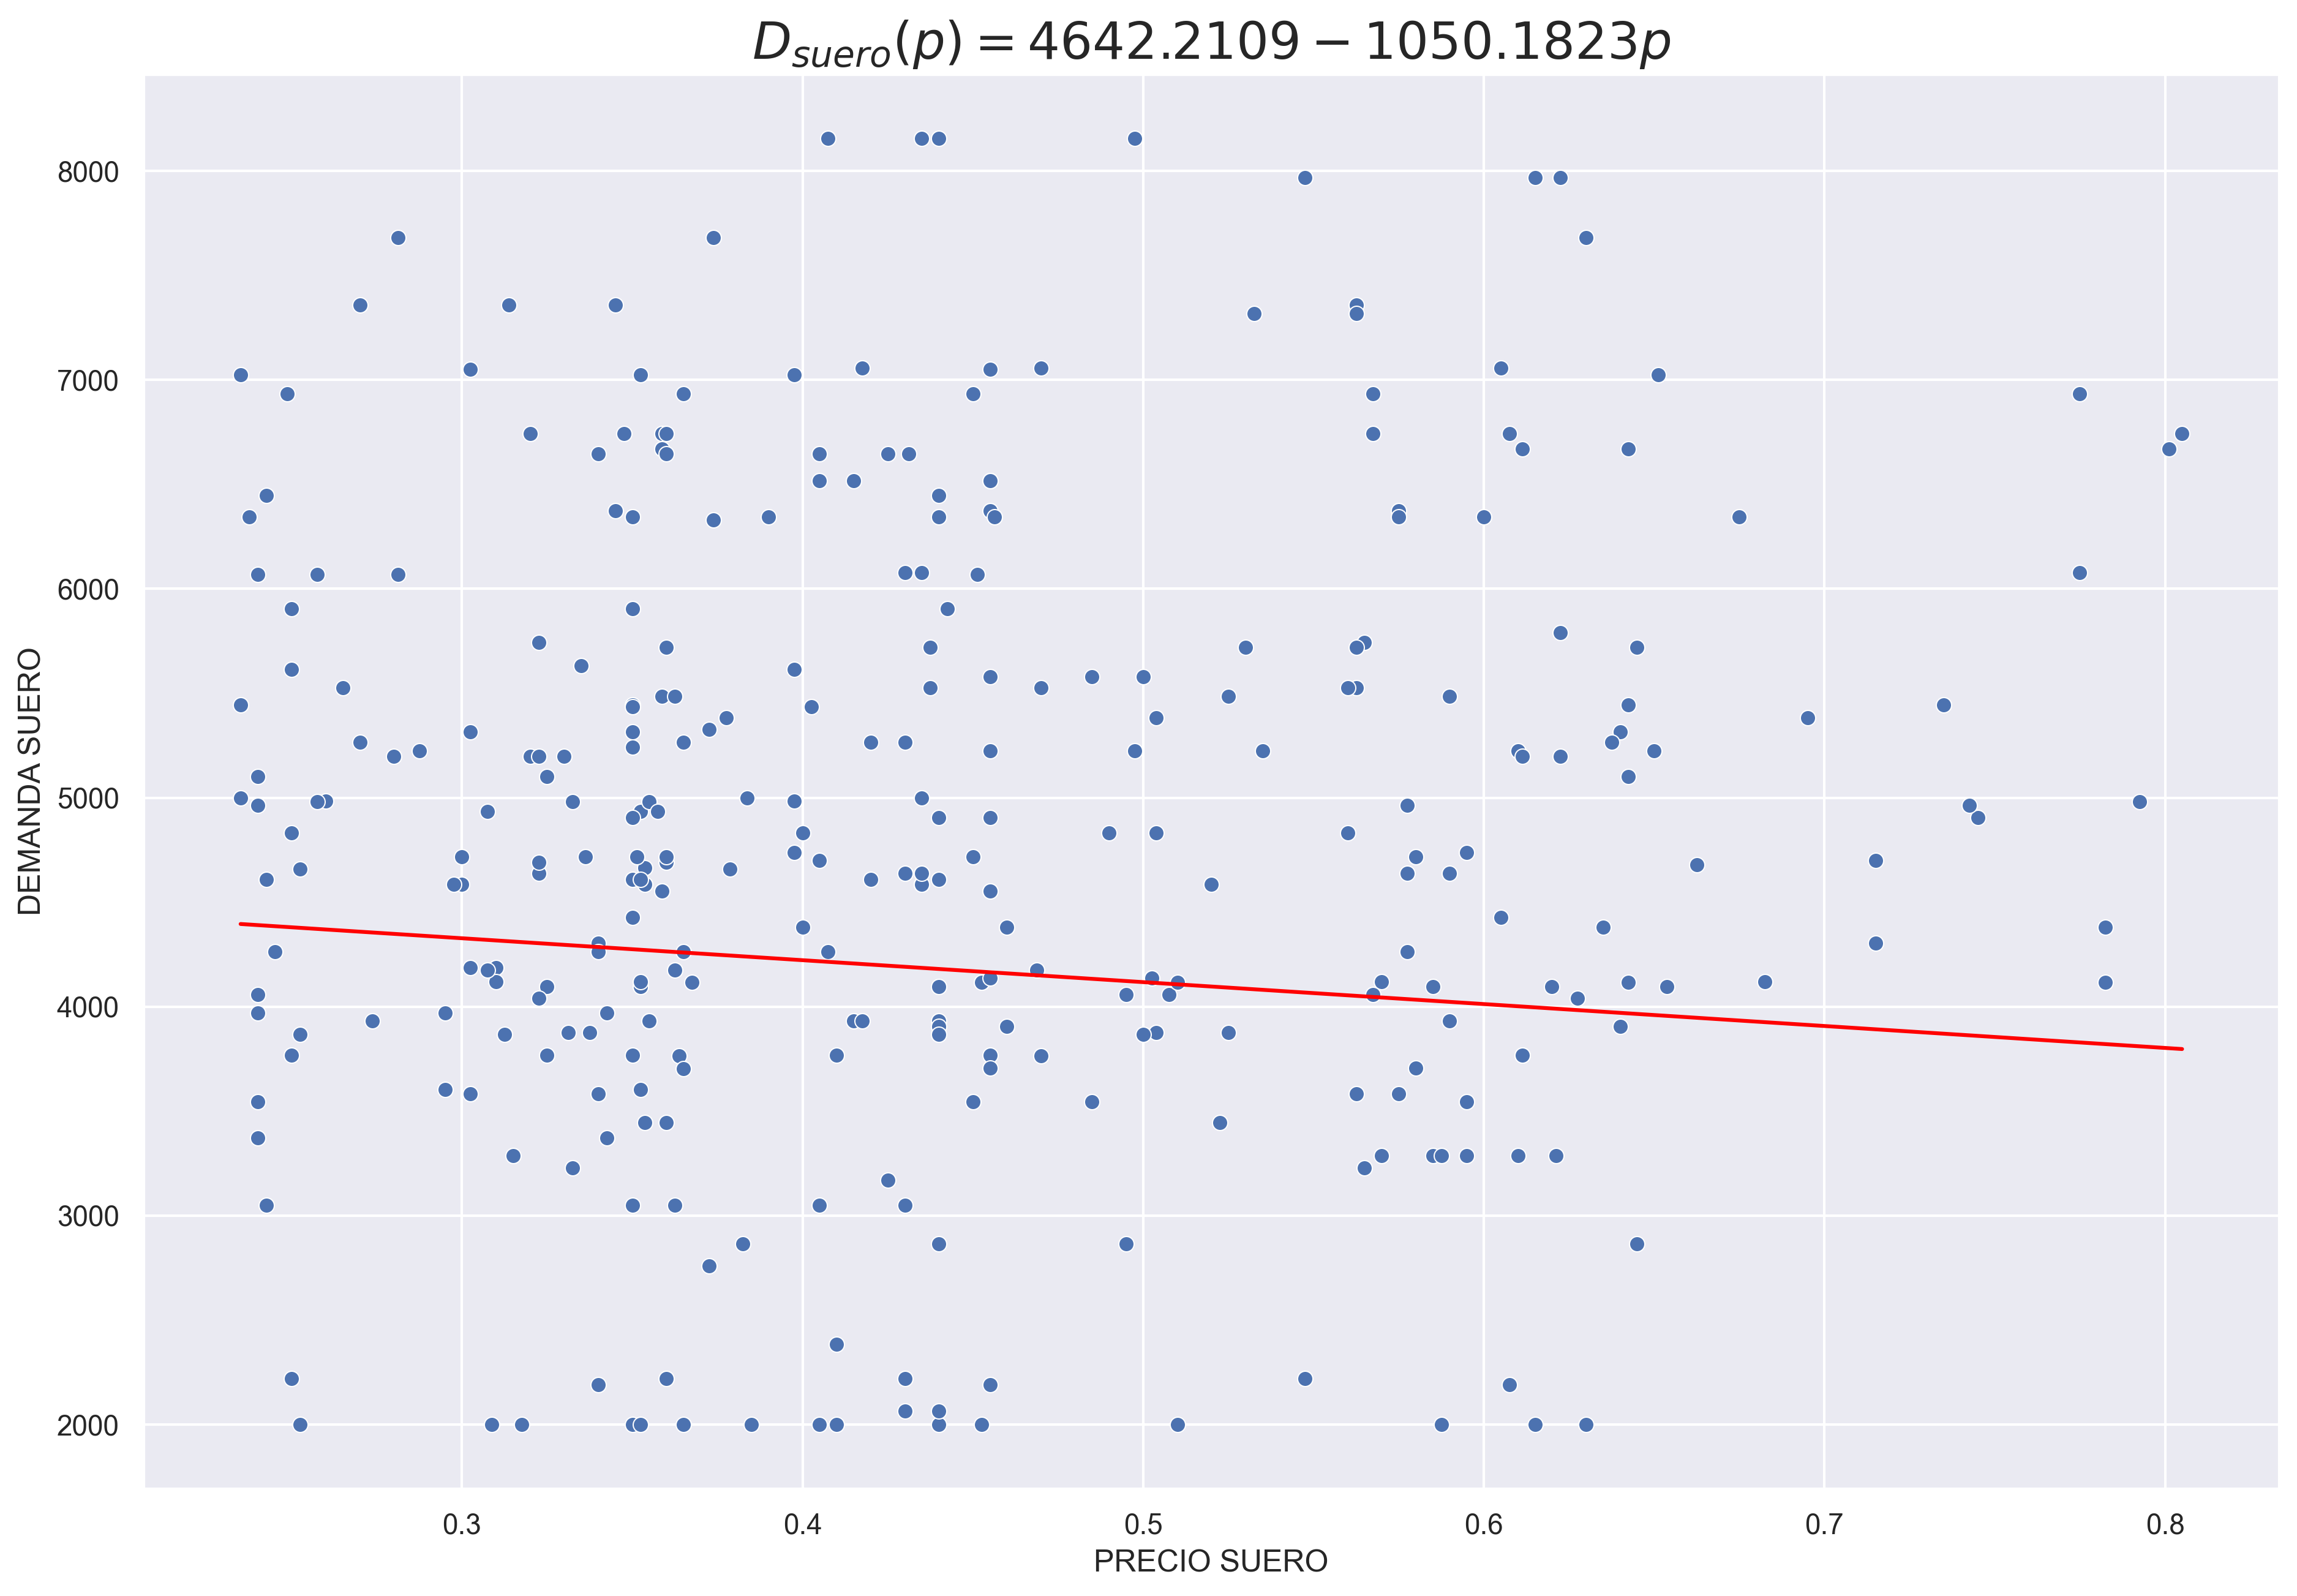
\includegraphics[width=0.7\textwidth]{demanda_suero}
\caption{Ecuación lineal ajustada a los datos sintéticos de demanda de suero.}
\label{fig:D_suero}
\end{figure}

\FloatBarrier
Las funciones de demanda determinadas anteriormente se utilizaron para implementar el modelo básico de optimización de precio, dando como resultado la Ecuacion \ref{eq:modLa} para la lactosa y la Ecuación \ref{eq:modSu} para el suero.

\begin{equation}\label{eq:modLa}
R_{lactosa}(p)=(p + p*0.10)*(4081.2654 - 1310.4058*(p + p*0.10))
\end{equation}

\begin{equation}\label{eq:modSu}
R_{suero}(p)=(p + p*0.10)*(4642.2109 - 1050.1823*(p + p*0.10))
\end{equation}

Al graficar dichas los modelos de optimzación de precio se puede observar que sí existe un punto máximo en el cuál las ganancias son las optimas, y podemos también tener una idea del espacio de búsqueda a considerar para encontrar dicho precio optimo. Esta gráfica de los modelos se muestra en la Figura \ref{fig:modelos}.

\begin{figure}[htbp]
\centering
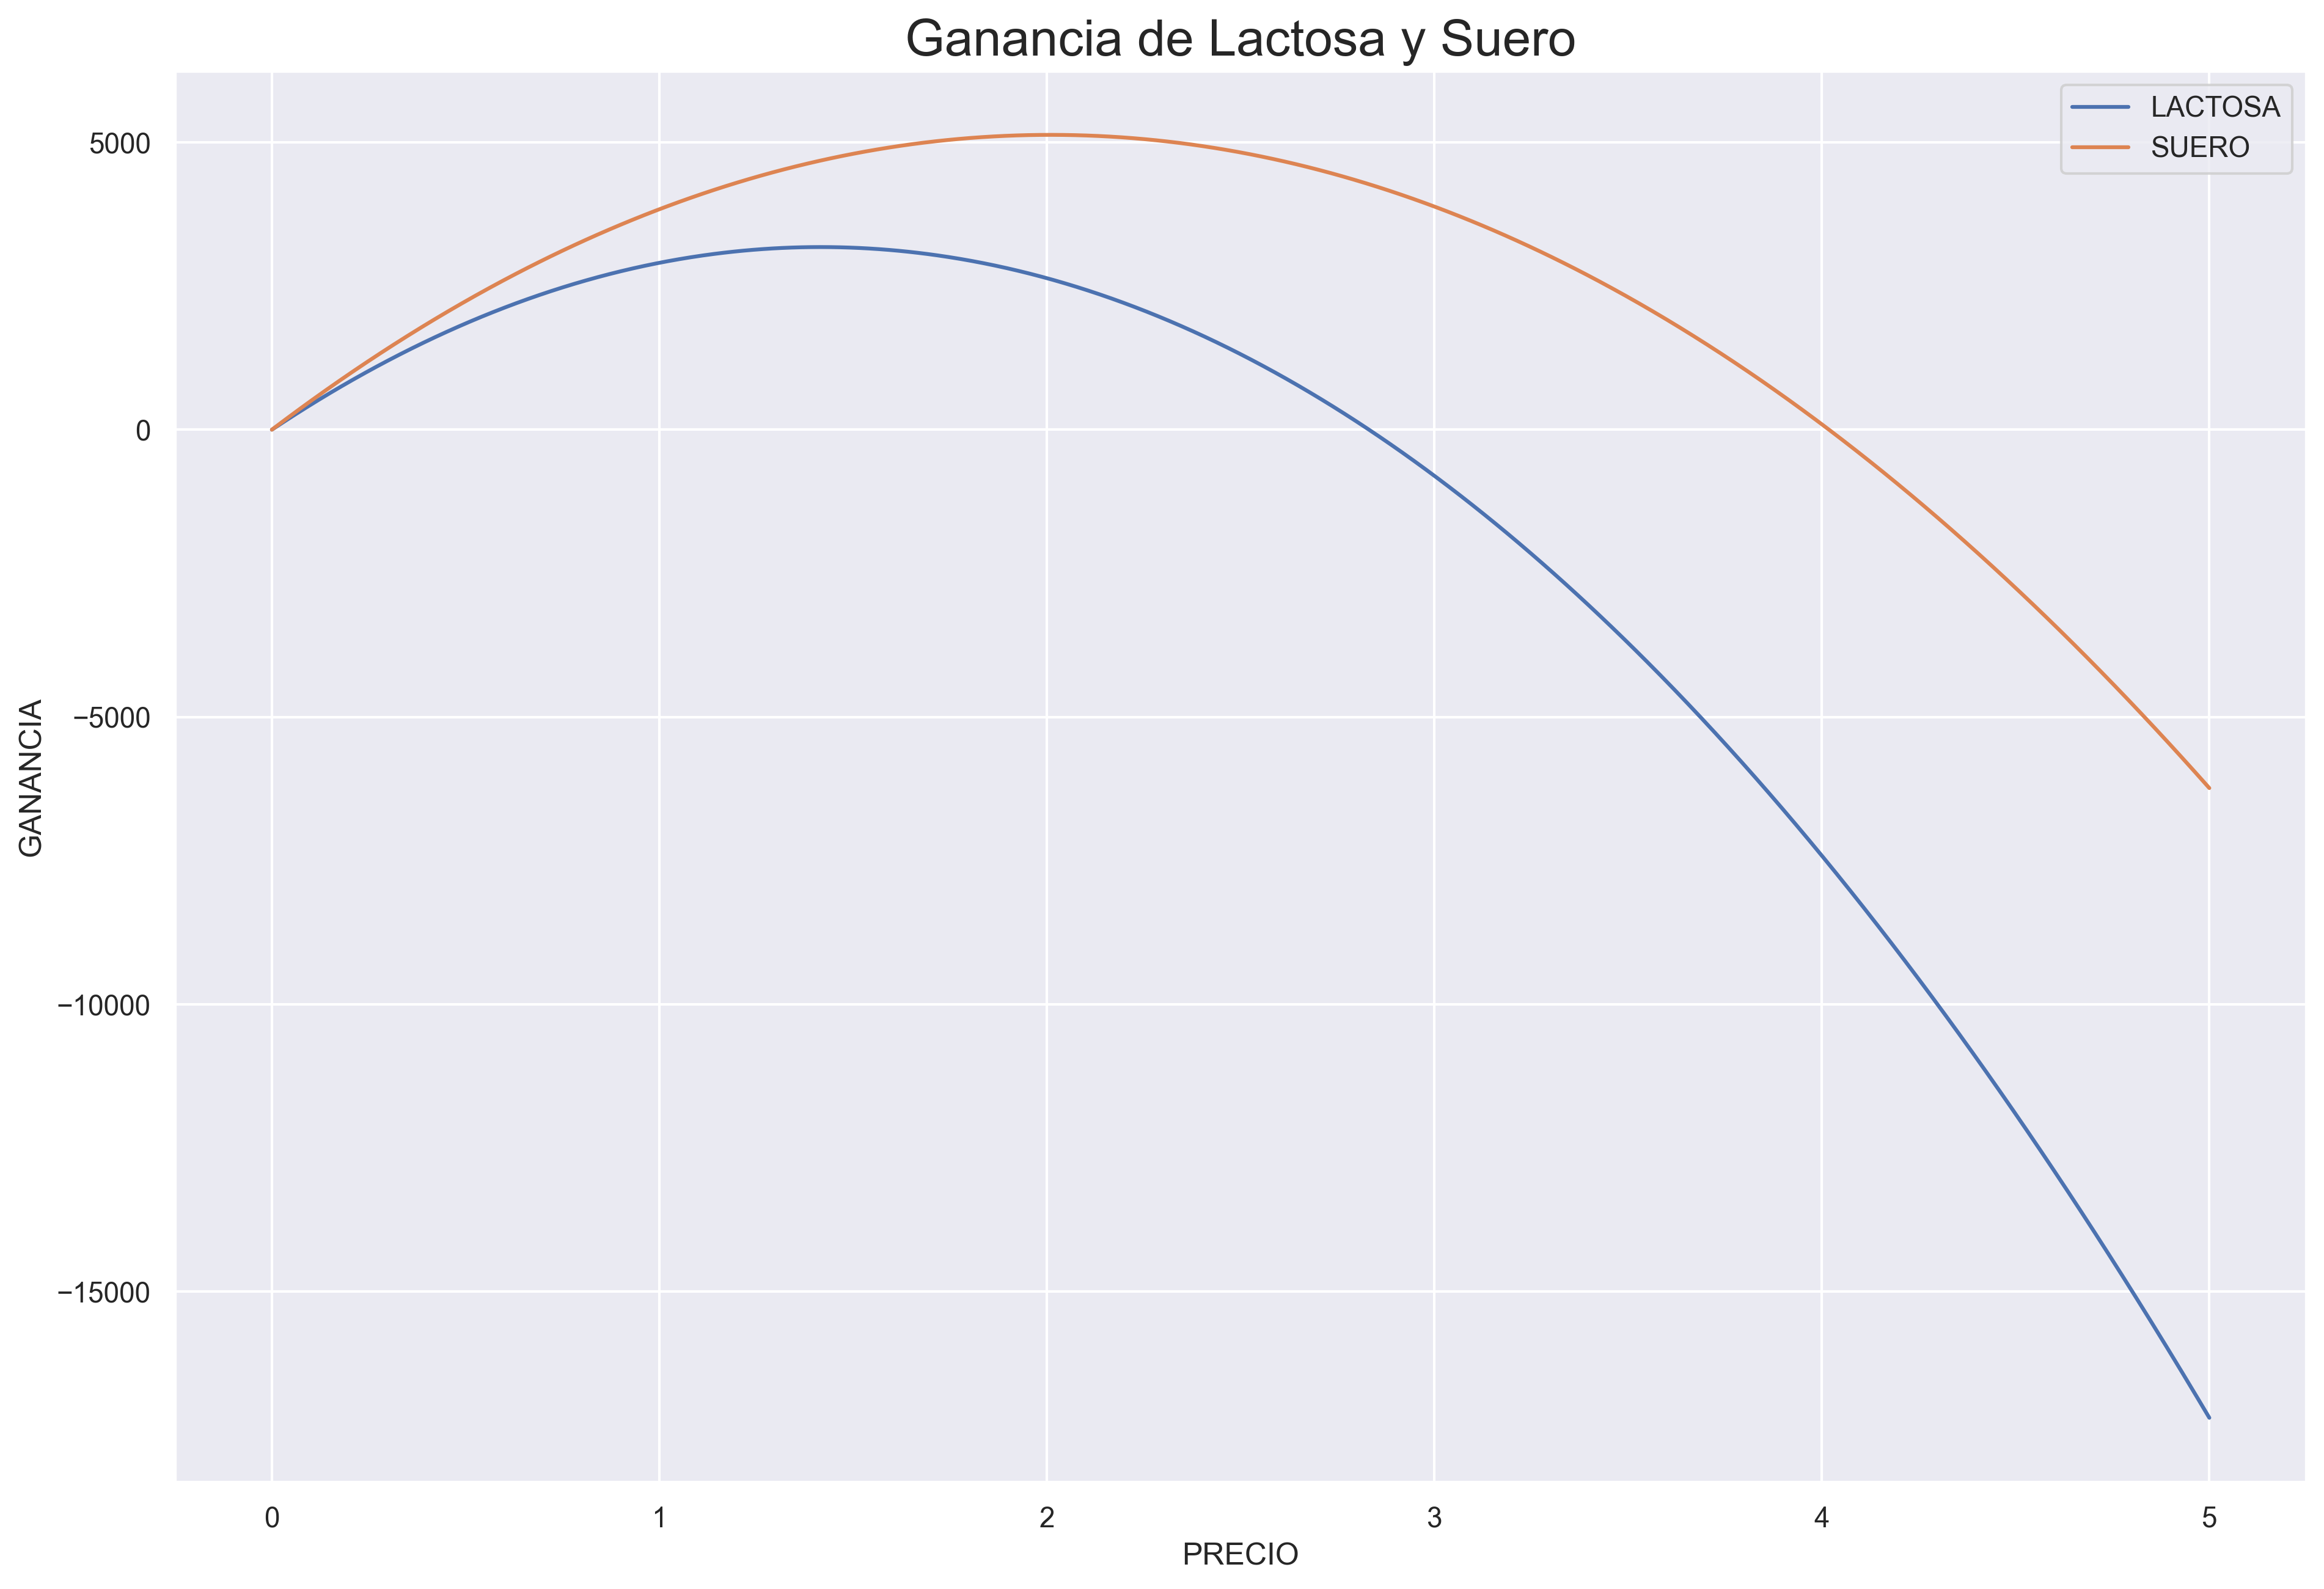
\includegraphics[width=0.7\textwidth]{revenue}
\caption{Modelos básicos de optimización de precio ante diferentes precios.}
\label{fig:modelos}
\end{figure}

\newpage
\subsection{Algoritmo genético}
Al optimizar el precio de cada uno de los productos utilizando un algoritmo genético se obtuvieron los resultados mostrados en las Figura \ref{fig:AG_la} y \ref{fig:AG_su}, donde se puede observar que en 8 generaciones se alcanza el precio optimo, el cual permite maximizar las ganancias de cada uno de los productos. 

\begin{figure}[htbp]
\centering
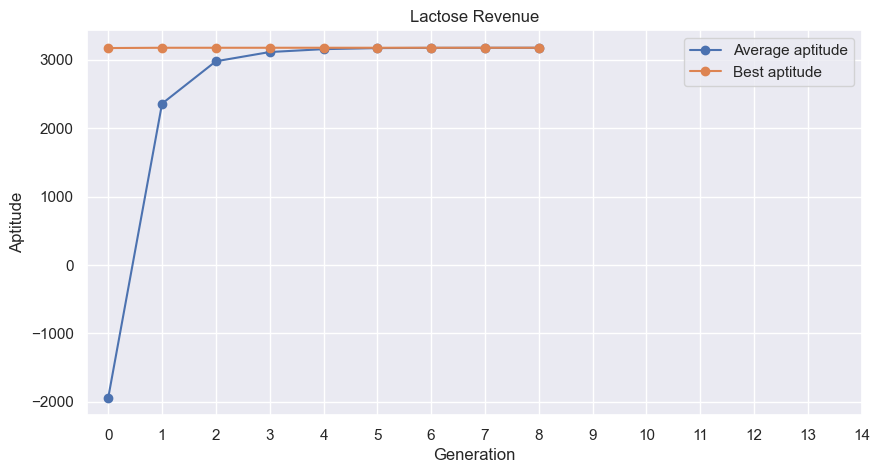
\includegraphics[width=0.7\textwidth]{lactose_revenue}
\caption{Evolución del algoritmo genético optimizador del precio de la lactosa.}
\label{fig:AG_la}
\end{figure}

\begin{figure}[htbp]
\centering
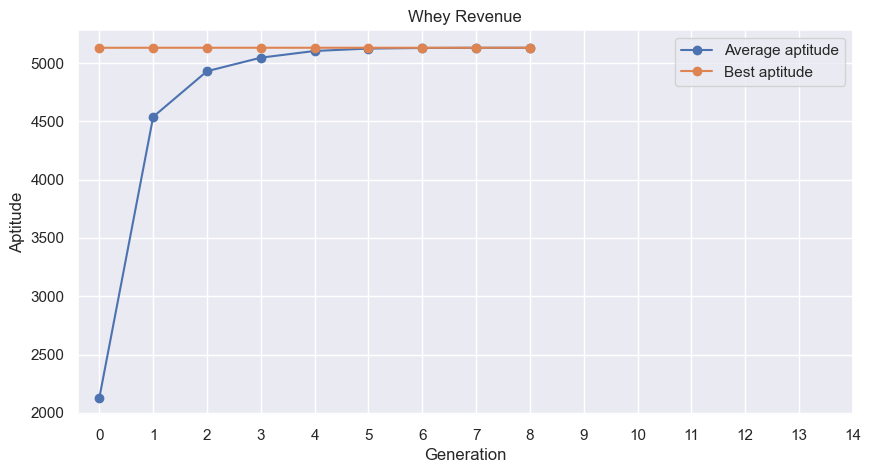
\includegraphics[width=0.7\textwidth]{whey_revenue}
\caption{Evolución del algoritmo genético optimizador del precio del suero.}
\label{fig:AG_su}
\end{figure}

\newpage
En cuanto al precio optimo para cada uno de los productos, la Tabla \ref{tab:precios} muestra el resultado de la última generación de cada algoritmo, donde se puede observar el precio optimo para cliente premium, el precio optimo para cliente estándar y la ganancia para clientes premium.

\begin{table}[htbp]
\centering
\caption{Precios finales y ganancia.}
\begin{tabular}{llll}
\hline
Producto & Ganancia   & Precio premium & Precio estándar \\ \hline
Lactosa  & 3,177.7799 & 1.3926         & 1.5318          \\
Suero    & 5,130.0906 & 2.0259         & 2.2284          \\ \hline
\end{tabular}
\label{tab:precios}
\end{table}
